\documentclass[10pt, a4paper]{report}

%\usepackage{fancyhdr}
\usepackage{hyperref}
\usepackage[T1]{fontenc}
\usepackage{ae,aecompl}
\usepackage{graphicx}
\usepackage[left=2cm, right=2cm, top=3cm, bottom=2.5cm]{geometry}
\usepackage{latexsym}
\usepackage{amsmath, amsthm, amssymb}
\usepackage{rotating}
\usepackage{boxedminipage}
\usepackage{multicol}

% Package for including code in the document
\usepackage{listings}

% If you want to generate a toc for each chapter (use with book)
% \usepackage{minitoc}

\begin{titlepage}
\title{Calcolo Numerico} 
\author{Massimo Nocentini}
\end{titlepage}
% My Theorem
\newtheorem{oss}{Osservation}[section]
\newtheorem{exercise}{Exercise}[section]
\newtheorem{thm}{Theorem}[section]
\newtheorem{cor}[thm]{Corollary}
\newtheorem{lem}[thm]{Lemma}


% page settings
\pagestyle{headings}

\begin{document}

% settings for the lstlisting environment
\lstset{
	language = octave
	, numbers = left 
	, basicstyle=\footnotesize
	, frame=single
	, tabsize=2
	, captionpos=b
	, breaklines=true
	, showspaces=false
	, showstringspaces=false
}

\maketitle

\tableofcontents

\newpage

\section*{Introduzione}
Queste note contengono tutto il mio materiale di studio per l'esame di Calcolo Numerico.

\subsection*{Sintassi esercizi}
Per gli esercizi utilizzo questa sintassi \textbf{Exercise n[(m)]}, dove $n$
rappresenta la numerazione locale all'interno delle sezioni di questo documento, 
$m$ rappresenta l'identificativo dell'esercizio fissato nel libro di testo 
\textbf{Calcolo Numerico} di \emph{Brugnano, Magherini, Sestini} pubblicato da \emph{Master}, 
prima edizione.
Il reference $(m)$ non \`e sempre presente, come evidenziato dall'uso delle parentesi quadre.



\chapter{Errori ed aritmetica finita}

\section{Discretizzazione} 

Questi errori sorgono tutte le volte che si vuole modellare un problema 
matematico (formulato nel continuo) con un sistema discreto. Per ottenere 
questo, uso dei processi di discretizzazione, dei quali mi interessa controllare
quanto ``bene'' approssimano il problema che voglio modellare.

Pi\`u specificamente, l'errore di troncamento \emph{locale} corrisponde 
all'errore introdotto nel passo di integrazione corrente assumendo esatto il 
valore di partenza, mentre l'errore di troncamento \emph{globale} rappresenta 
l'effetto di tutti gli errori precedenti.

Per i seguenti due esercizi si utilizza la formula di Taylor-Peano, con il 
resto ''infinitesimo di ordine superiore'' rispetto al massimo grado $n$ a cui 
si arresta lo sviluppo e quindi consente di ottenere una approssimazione
locale, cio\`e in un intorno di $x_{0}$.

\begin{exercise}[1.1]
	Sia $x = \pi \approx 3.14159265$. Considero come valore approssimato 
	$\tilde{x} = 3.1415$. 
	
	Calcolare il corrispondente errore relativo\footnote{D\'a l'ordine di 
	grandezza rispetto alla base $10$} $\varepsilon_{x}$. 
	
	Verificare che il numero di cifre decimali corrette nella rappresentazione 
	approssimata di $x$ mediante $\tilde{x}$ all'incirca \`e dato da $-\log_{10}
	{|\varepsilon_{x}|}$.
\end{exercise}
Ottengo:
\begin{displaymath}
	\varepsilon_{x} = \frac{\tilde{x}-x}{x} = \frac{3.1415-3.14159265358979}
	{3.14159265358979}
\end{displaymath}
\begin{lstlisting}
octave:19> (3.1415-pi)/pi
ans = -2.94925536215087e-05
\end{lstlisting}
Adesso considero:
\begin{equation*}
	-\log_{10}{|-2.9491 \times 10^{-5}|} = -\left (\log_{10}{2.9491} +
	\log_{10}{10^{-5}} \right ) = -\log_{10}{2.9491} + 5\log_{10}{10}
\end{equation*}
\begin{lstlisting}
octave:18> -log10(2.9491) + 5*log10(10)
ans =  4.53031050085890e+00
\end{lstlisting}
L'approssimazione $\tilde{x}$ ha 4 cifre decimali corrette.

\begin{exercise}
Dimostrare che $-\log_{10}{|\varepsilon_{x}|}$ d\`a all'incirca il numero 
di cifre decimali corrette di $\tilde{x}$, con cui approssimo $x$. 
\end{exercise}
\begin{proof}
Sia $r$ il numero di cifre decimali \emph{esatte}, tale che 
$r = -\log_{10}{|\varepsilon_{x}|}$. Passando agli esponenti ottengo 
$|\varepsilon_{x}| = 10^{-r}$.

Dato che cerco un'approssimazione del numero di cifre decimali a partire dall'
errore relativo, imposto due disequazioni per trovare un intervallo in cui $r$
pu\`o variare.

Scrivo in forma normalizzata il valore esatto $x$ e la sua approssimazione 
$\tilde{x}$, fissando $\beta = 10$ e $M \not = m$ perch\`e sto approssimando:
\begin{equation*}
	\begin{split}
		x \in \mathbb{R}, x \geq 0, x = m \times 10^{e} \\
		\tilde{x} \in \mathbb{R}, \tilde{x} \geq 0, \tilde{x} = M \times 10^{e}
	\end{split}
\end{equation*}
Per il \emph{teorema 1.2} vale $ 1 \leq m < 10 \wedge  1 \leq M < 10$.

Adesso voglio trovare sia una maggiorazione che una minorazione di 
$\varepsilon_{x}$:
\begin{equation*}
	\left | \varepsilon_{x} \right | = \left | \frac{(M - m) \times 10^{e}} 
		{m \times 10^{e}}
	\right | = \left | \frac{M - m}{m} \right |
\end{equation*}
Maggioro con:
\begin{equation*}
	\left | \frac{M - m}{m} \right | < 10 = max
\end{equation*}
In quanto il massimo lo ottengo quando $M = 9, m = 1$.

Minoro con:
\begin{equation*}
	min = \frac{1}{10} \le \left | \frac{M - m}{m} \right | 
\end{equation*}
In quanto il minimo lo ottengo quando $M = 8, m = 9$.

Adesso posso impostare le due disequazioni:
\begin{equation*}
	10^{-r -1} = \frac{\left | \varepsilon_{x} \right |}{10} \le 
		\left | \varepsilon_{x} \right | <
	10 \left | \varepsilon_{x} \right | = 10^{-r +1}
\end{equation*}
Le uguaglianze esterne valgono per quanto detto ad inizio prova.
%10^{-r-1} \leq |\varepsilon_{x}| < 10^{-r+1}
Passo ai logaritmi:
\begin{equation*}
	\begin{split}
		-r-1 \leq  \log_{10}{|\varepsilon_{x}|} < -r+1 \\
		r+1 \geq -\log_{10}{|\varepsilon_{x}|} > r-1
	\end{split}
\end{equation*}
Considero i rami $-r-1 \leq  \log_{10}{|\varepsilon_{x}|}$ dalla prima e 
$-\log_{10}{|\varepsilon_{x}|} > r-1$ dalla seconda per avere l'intervallo di variazione di $r$:
\begin{equation*}
	-1 - \log_{10}{|\varepsilon_{x}|} \leq r < 1 - \log_{10}{|\varepsilon_{x}|}
\end{equation*}
\end{proof}

\begin{exercise}[1.2]
	Dimostrare che, se $f(x)$ \`e sufficientemente regolare e $h>0$ \`e una 
	quantit\`a piccola, allora:
	\begin{equation*}
		\begin{split}
			\frac{f(x_{0}+h) - f(x_{0}-h)}{2h} =& f'(x_{0}) + O(h^{2}), \\
			\frac{f(x_{0}+h) - 2f(x_{0}) + f(x_{0}-h)}{h^{2}} =& f''(x_{0}) + O(h^{2}) 
		\end{split}
	\end{equation*}
\end{exercise}
Per entrambe considero gli sviluppi di Taylor di $f(x_{0}+h)$ e $f(x_{0}-h)$ in
$x_{0}$:
\begin{equation*}
	\begin{split}
		T(x_{0} + h)& = f(x_{0}) + f'(x_{0})h + \frac{f''(x_{0})h^{2}}{2} + 
		\frac{f'''(x_{0})h^{3}}{6} + O(h^{4}) \\ 
		T(x_{0} - h)& = f(x_{0}) - f'(x_{0})h + \frac{f''(x_{0})h^{2}}{2} - 
		\frac{f'''(x_{0})h^{3}}{6} + O(h^{4})
	\end{split}
\end{equation*}
Devo prestare attenzione al segno di alcuni termini dello sviluppo
\footnote{Attenzione: nello sviluppo di Taylor di una funzione $f(x)$,  le
derivate $n$-esime vengono calcolate nel punto $x_{0}$ in cui si vuole 
centrare lo sviluppo, e non nell'argomento della funzione}:
\begin{itemize}
	\item nel primo sviluppo, la combinazione lineare ammette tutti segni 
	positivi in quanto il passo di discretizzazione \`e positivo, ovvero si cerca
	di approssimare con valori $ > x_{0}$.
	\item nel secondo invece, il fattore $((x_{0} - h - x_{0} =h))^{k} < 0, 
	\forall{k=2n+1, n \in \mathbb{N}}$ fa si che i termini dello sviluppo di 
	grado dispari siano negativi, in quanto si sta discretizzando con un valore 
	minore a $x_{0}$, di conseguenza $x - x_{0} < 0$.
\end{itemize}
Sottraendo termine a termine e semplificando dove possibile ottengo la prima equazione: 
\begin{equation*}
	T(x_{0}+h) - T(x_{0}-h) = 2f'(x_{0})h + \frac{f'''(x_{0})h^{3}}{3} + O(h^{4}) 
\end{equation*}
dividendo per $2h$: 
\begin{equation*}
	\frac{T(x_{0}+h) - T(x_{0}-h)}{2h} = f'(x_{0}) + \frac{f'''(x_{0})h^{2}}{3}  +
	O(h^{3})
\end{equation*}
Osserviamo che, per $h \rightarrow 0$, la quantit\`a $O(h^{3})$ diminuisce pi\`u 
velocemente del termine $$\frac{f'''(x_{0})h^{2}}{3}$$ per cui possiamo dedurre
che si approssima la derivata prima con una quantit\`a $O(h^{2})$.

Per la seconda equazione invece che sottrarre termine a termine, sommiamo,
ottenendo:
\begin{equation*}
	\begin{split}
		T(x_{0}+h) + T(x_{0}-h) = 2f(x_{0}) + f''(x_{0})h^{2} + O(h^{4})\\
		\frac{T(x_{0}+h) - 2f(x_{0}) + T(x_{0}-h)}{h^{2}} = f''(x_{0}) + O(h^{2}) 
	\end{split}
\end{equation*}
ovvero la quantit\`a al primo membro approssima la $f''(x_{0})$ con un errore 
dell'ordine $O(h^{2})$.

\section{Errori di convergenza}

\begin{exercise}[1.3] 
\label{exercise:exerciseIterativeMethodFixedPoint}
Dimostrare che il metodo iterativo $$x_{n+1}=\phi(x_{n})$$ convergente a x*,
deve verificare la condizione di \textbf{consistenza} $$x^{*}=\phi(x^{*})$$
ovvero la soluzione cercata deve essere un punto fisso per la funzione di
iterazione che definisce il metodo.
\end{exercise}
\begin{proof}
Suppongo che il metodo $\phi$ sia monotono e convergente a $x^{*}$. Definisco
il preordine $\rightarrow$ per catturare la convergenza:
\begin{displaymath}
\rightarrow = \lbrace (x_{n}, x_{n+1}) : x_{n+1} = \phi(x_{n}) \wedge \lim_{n
\rightarrow \infty}{x_{n}} = x^{*}
\rbrace
\end{displaymath}
Suppongo \emph{per assurdo} che $$\phi(x^{*}) = x^{\triangle} \not = x^{*}$$
Per l' ipotesi $x_{n} \rightarrow x^{*}$ (per la transitivit\`a di
$\rightarrow$), posso applicare la monotonia di $\phi$ rispetto a $\rightarrow$:
$$\phi(x_{n}) \rightarrow \phi(x^{*}) = x^{\triangle}$$ ma questo contraddice 
l'ipotesi che $\phi$ converge a $x^{*}$.
\end{proof}

\begin{exercise}
Considerare il metodo iterativo:
\begin{displaymath}
	x_{n+1} = \phi(x_{n}) = \frac{1}{2} \left ( x_{n} + \frac{2}{x_{n}} \right ), 
		\quad x_{0} = 2
\end{displaymath}
dimostrare che il metodo genera una successione di approssimazioni tale che 
$x_{n} \rightarrow \sqrt{2}$.
\end{exercise}
\begin{proof}
Questo metodo \`e a passo \emph{singolo} in quanto usa un solo innesto per calcolare
$x_{n + 1}$.
Affinch\`e il metodo iterativo sia convergente, per l'esercizio 
\ref{exercise:exerciseIterativeMethodFixedPoint} posso costruire
un'equazione per trovare il punto fisso di $\phi$:
\begin{displaymath}
\phi(x) = \frac{1}{2} \left ( x + \frac{2}{x} \right ) = x
\end{displaymath}
Manipolando: $x + \frac{2}{x} = 2x \Rightarrow x^{2} + 2 = 2x^{2} \Rightarrow 
	2 = x^{2}$
\end{proof}

\begin{exercise}[1.4] Per il testo dell'esercizio consultare il libro di testo.
\end{exercise}
Eseguendo il codice riportato nella sezione \nameref{sec:iterativeMethodToSQRT2}, 
questo \`e l'output di Octave sulla mia macchina:
\begin{lstlisting}
octave:8> iterative(2, 1.5)
next =  1.42857142857143e+00
Difference with last step:0.0714285714285714
next =  1.41463414634146e+00
Difference with last step:0.0139372822299655
next =  1.41421568627451e+00
Difference with last step:0.000418460066953008
next =  1.41421356268887e+00
Difference with last step:2.12358564088966e-06
next =  1.41421356237310e+00
Difference with last step:3.15774073555986e-10
Difference with sqrt(2):0
\end{lstlisting}
In 5 passi si raggiunge la precisione richiesta, uno in pi\`u rispetto ai risultati
mostrati in \emph{Tabella 1.1} del libro.




\section{Errori di round-off}

\chapter{Radici di una equazione}

\section{Metodi iterativi}

\begin{exercise}[2.2]
	Per il testo dell'esercizio consultare il libro di testo.
\end{exercise}
Il metodo da trovare deve convergere a $x^{*} = \sqrt[m]{a}$ che, per l'esercizio
\ref{exercise:exerciseIterativeMethodFixedPoint}, deve verificare la condizione 
di consistenza:
\begin{displaymath}
	x^{*}=\phi(x^{*}), \quad \quad \phi(x^{*}) = x^{*} - 
		\frac{f(x^{*})}{f'(x^{*})}
\end{displaymath}
Implementando con $\phi$ il metodo di Newton che si chiede di usare.
Unendo le due uguaglianze sopra si ottiene:
\begin{equation}
\label{equation:equalsToZeroRequirement}
\begin{split}
	x^{*} &= x^{*} - \frac{f(x^{*})}{f'(x^{*})} \\
	0 &= f(x^{*})
\end{split}
\end{equation}
La (\ref{equation:equalsToZeroRequirement}) mi da un vincolo per la ricerca
della $f$. Posso adesso sfruttare la richiesta di convergenza:
\begin{equation}
\begin{split}
	x &= \sqrt[m]{a} \\
	f(x) = x^{m} - a &= 0
\end{split}
\end{equation}
Ho quindi costruito una funzione che rispetta il vincolo espresso nella
(\ref{equation:equalsToZeroRequirement}). Scrivo il metodo iterativo:
\begin{displaymath}
\begin{split}
	x_{i+1} &=\phi(x_{i}) \\
	\phi(x_{i}) &= x_{i} - 
		\frac{x_{i}^{m} - a}{m x_{i}^{m - 1}} = 
		\frac{m x_{i}^{m} - x_{i}^{m} + a}{m x_{i}^{m - 1}} = \\
	&= 	\frac{(m - 1) x_{i}^{m} + a}{m x_{i}^{m - 1}} = 
			\frac{m - 1}{m} x_{i} + \frac{a}{m x_{i}^{m - 1}}
\end{split}
\end{displaymath}
Verifico adesso che il metodo rispetti la condizione necessaria per la convergenza.
\begin{proof}
Per l'esercizio \ref{exercise:exerciseIterativeMethodFixedPoint} vale:
\begin{equation}
\begin{split}
	x &= \frac{m - 1}{m} x + \frac{a}{m x^{m - 1}} \\
	m x^{m} &= (m - 1) x^{m} + a \\
	x^{m} (m + 1 - m) &= a \\
	x^{m} &= a \\
\end{split}
\end{equation}
Il metodo $\phi$ soddisfa la condizione necessaria, converge al valore
richiesto e questo termina la prova.
\end{proof}

\begin{exercise}[2.3]
Per il testo dell'esercizio consultare il libro di testo.
\end{exercise}
Per la definizione del metodo delle secanti vale:
\begin{displaymath}
	x_{i + 1} = \frac{f(x_{i})x_{i-1} - f(x_{i-1})x_{i}}{f(x_{i}) - f(x_{i-1})}
\end{displaymath}
Come per l'esercizio precedente, devo verificare che il metodo soddisfi la
condizione necessaria di convergenza \footnote{qui mi \`e difficile far vedere
che vale la condizione necessaria, in quanto si annulla il denominatore}.
La verifica fornisce un vincolo per la funzione $f$ da ricercare: $f(x) = 0$, 
quindi agisco come nell'esercizio precedente, considerando la richiesta di
convergenza:
\begin{equation}
\begin{split}
	x &= \sqrt{a} \\
	f(x) = x^{2} - a &= 0
\end{split}
\end{equation}
Posso adesso sostituire nella definizione del metodo:
\begin{displaymath}
\begin{split}
	x_{i + 1} &= \frac{(x_{i}^{2} - a)x_{i-1} - (x_{i-1}^{2} - a)x_{i}}
		{x_{i}^{2} - a - (x_{i-1}^{2} - a)}
			  = \frac{x_{i}^{2} x_{i-1} - a x_{i-1} - 
						x_{i-1}^{2} x_{i} + a x_{i}}
					{x_{i}^{2} - x_{i-1}^{2}} = \\
			  &= \frac{a(x_{i} - x_{i-1}) + x_{i}x_{i-1}(x_{i} - x_{i-1})}
					{(x_{i} - x_{i-1})(x_{i} + x_{i-1})} 
			  = \frac{(x_{i} - x_{i-1})(a + x_{i}x_{i-1})}
					{(x_{i} - x_{i-1})(x_{i} + x_{i-1})} 
			  = \frac{a + x_{i}x_{i-1}}{x_{i} + x_{i-1}}
\end{split}
\end{displaymath}
Verifico che il metodo caratterizzato soddisfi la condizione necessaria di
convergenza.
\begin{proof}
Per l'esercizio \ref{exercise:exerciseIterativeMethodFixedPoint} vale:
\begin{displaymath}
\begin{split}
\lim_{i\rightarrow\infty}{x_{i}} = x^{*} & = \sqrt{a} \quad\Rightarrow \quad
x_{i+1} = x_{i} = x_{i-1} = x, \quad \text{segue che} \\
x &= \frac{a + x^{2}}{2x} \\ 
2x^{2} &= a + x^{2} \\
x^{2} &= a
\end{split}
\end{displaymath}
E questo termina la prova.
\end{proof}
Comparando con l'\emph{Esercizio 1.4} del libro di testo si vede che il metodo
proposto in tale esercizio \`e la caratterizzazione del metodo delle secanti 
qui discusso con la caratterizzazione di $a = 2$:
\begin{displaymath}
x_{i + 1} = \frac{2 + x_{i}x_{i-1}}{x_{i} + x_{i-1}}
\end{displaymath}

\begin{oss}[Sul teorema di punto fisso]
Se parto da due punti nell'intervallo $x, y \in I = (x^{*} - \delta, x^{*} +
\delta)$, allora applicando il metodo iterativo $\phi$ ai due punti ottengo una
nuova coppia $\phi(x) = x_{1}, \phi(y) = y_{2}$, la cui distanza $|x_{1} - y_{1}|$
\`e strettamente minore della distanza dei punti di partenza in quanto $L < 1$
per ipotesi del teorema: ottengo quindi $|x_{1} - y_{1}| < |x - y|$. In questo
modo sono riuscito ad ottenere una nuova coppia di punti pi\`u vicina.

Questo \`e quello che avrei voluto in quanto una volta applicato il metodo ad
una coppia, ottengo una coppia di punti pi\`u vicina: se riesco ad applicare
nuovamente il metodo alla coppia appena costruita riuscirei ad ottenere una
nuova coppia di punti pi\`u vicini rispetto alla ultima coppia generata.
Ripetendo un numero sufficiente di volte il metodo $\phi$ riesco a diminuire la
distanza tra i punti delle coppie, fino a far degenerare una coppia di punti
distinti allo stesso punto $(x_{k}, x_{k})$, ovvero al punto fisso del metodo,
e quindi convergere alla soluzione.

Importante quindi \`e partire da una coppia di punti che appartengono
all'intervallo $I$ per poter applicare almeno una volta il metodo.

Posso commentare le implicazioni del teorema:
\begin{enumerate}
  \item $x^{*}$ \`e l'unico punto fisso di $\phi$ in $I$: questo permette al
  metodo di non oscillare tra due punti fissi (soluzioni) e inoltre di non
  creare non determinismo nella scelta della soluzione a cui converge il metodo
  \item se $x_{0} \in I \Rightarrow \phi(x_{i-1}) = x_{i} \in I, \forall i =
  \{2, 3, \ldots\}$: questo \`e molto importante perch\`e assicura che ogni
  punto generato dal metodo $\phi$ appartiene all'intervallo se il punto di
  innesco $x_{0} \in I$. In questo modo, tornando a ragionare per coppie come
  fatto nei paragrafi precedenti di questa osservazione, se il punto di innesco
  appartiene all'intervallo $I$ allora tutti i nuovi punti che posso costruire
  con il metodo $\phi$ apparterranno anch'essi all'intervallo e quindi posso 
  ragionare a coppie $(x_{i-1}, x_{i})$ e applicare il teorema ad ogni coppia
  per $i \in \{ 1, 2,\ldots \}$, ottenendo quindi che i punti della coppia
  $(x_{i}, x_{i+1})$ saranno pi\`u vicini dei punti della coppia $(x_{i-1},
  x_{i})$.
  \item $\lim_{i \rightarrow \infty}{x_{i}} = x^{*}$, ovvero il metodo converge
  alla soluzione $x^{*}$ punto fisso di $\phi$ per la condizione necessaria.
\end{enumerate}
\end{oss}

\begin{exercise}
 Dire se il seguente metodo iterativo \`e convergente e se si a quale punto
 converge.
 \begin{displaymath}
 	x_{k+1} = \sqrt{x_{k} + 1}
 \end{displaymath}
\end{exercise}
Formalizzo il metodo con la funzione $\phi$:
\begin{displaymath}
 	\phi(x) = \sqrt{x + 1}
 \end{displaymath}
Se il metodo converge, per la condizione necessaria, converge al suo punto
fisso, quindi lo determino:
\begin{displaymath}
 \begin{split}
 	x &= \phi(x) = \sqrt{x + 1} \\
 	x^{2} &= x + 1 	
 \end{split}
\end{displaymath}
Implica che le due soluzioni sono $x_{1,2} = \frac{1 \pm \sqrt{5}}{2}$.

Non ho dimostrato che il metodo converge, ho solo trovato il punto di
convergenza se il metodo converge. Dimostro adesso la convergenza controllando
che siano vere le ipotesi del teorema di punto fisso:
\begin{displaymath}
 \begin{split}
 	\exists \delta > 0 \exists l, 0 \leq l < 1 &: \forall x, y \in I = (x^{*} -
 	\delta, x^{*} +	\delta): \\
 	|\phi(x) - \phi(y)| &< l|x - y|
 \end{split}
\end{displaymath}
Dato che $\phi$ \`e derivabile allora sviluppo $\phi(y)$ in $x$ con resto al
primo ordine, per applicare il metodo due volte nello stesso punto:
\begin{displaymath}
 \begin{split}
 	T_{\phi(y)}(x) = \phi(x) + \phi'(\xi)(y - x), \quad \xi \in [x, y]
 	(\Rightarrow \xi \in I)
 \end{split}
\end{displaymath}
Posso sostituire nella precedente disuguaglianza:
\begin{displaymath}
 \begin{split}
 	|\phi(x) - \phi(x) + \phi'(\xi)(y - x)| &< l|x - y| \\
 	|\phi'(\xi)(y - x)| &< l|x - y| \\
 	|\phi'(\xi)||x - y| &< l|x - y| \\
 	|\phi'(\xi)| &< l < 1
 \end{split}
\end{displaymath}
Devo quindi verificare:
\begin{displaymath}
 \begin{split}
 	|\phi'(\xi)| &< 1 \\
 	\phi'(x) &= \frac{1}{2\sqrt{x + 1}} \\
 	\frac{1}{2\sqrt{x + 1}} &< 1 \\
 	1 &< 2\sqrt{x + 1}, \forall x \geq 0
 \end{split}
\end{displaymath}
Sono nelle ipotesi del teorema di punto fisso \footnote{l'unica cosa che rimane
da trovare \`e $l$} quindi per l'implicazione del teorema valgono
\begin{itemize}
  \item $x = \frac{1 \pm \sqrt{5}}{2}$ \`e l'unico punto fisso di $\phi$ in $I$
  \item tutti i punti $x_{i}$ generati dal metodo appartengono all'intervallo
  $I$
  \item il metodo converge a $x = \frac{1 \pm \sqrt{5}}{2}$.
\end{itemize}

\section*{Metodi con rappresentazione grafica}
I prossimi metodi che verranno descritti utilizzeranno lo strumento Octave
per la rappresentazione grafica dei metodi per illustrare in modo pi\`u chiaro
il comportamento del metodo iterativo in questione.

Tutti i grafici hanno uno schema comune, ovvero sono composti da tre curve:
\begin{itemize}
  \item la curva cyan rappresenta la funzione $f(x)$ che si sta studiando
  \item la curva blu, composta da pochi simboli '$+$', rappresenta punti
  calcolati dal metodo per convergere allo zero $x^{*}$
  \item la curva rossa rappresenta il comportamento del metodo, visualizzando
  la sequenza con cui si procede per convergere alla soluzione
\end{itemize}

\section{Metodo di bisezione}
\label{sec:metodoDiBisezione}
Riporto il codice di pagina 23:
\begin{lstlisting}
octave:12> p = poly([1.1*ones(1,20) pi])
p =
 Columns 1 through 6:
   1.0000e+00  -2.5142e+01   2.9902e+02  -2.2396e+03   1.1860e+04  -4.7254e+04
 Columns 7 through 12:
   1.4711e+05  -3.6678e+05   7.4461e+05  -1.2444e+06   1.7234e+06  -1.9847e+06
 Columns 13 through 18:
   1.9008e+06  -1.5096e+06   9.8794e+05  -5.2718e+05   2.2572e+05  -7.5702e+04
 Columns 19 through 22:
   1.9159e+04  -3.4410e+03   3.9100e+02  -2.1135e+01
octave:13> polyval(p,pi)
ans =  2.0207e-04
\end{lstlisting}
Lo scopo della funzione $poly(r)$ \`e quello di creare un vettore di coefficienti
di un polinomio $p$, tale che le radici di $p$ appartengono al vettore $r$ 
($poly: Root[] \rightarrow PolynomialCoefficient[]$).
Valutando quindi il polinomio in una sua radice (\emph{octave:13}) in aritmetica
esatta dovrei ottenere 0, mentre in aritmetica finita non \`e vero 
($p(\pi) = ans =  2.0207e-04 \not = 0$).

\begin{exercise}
Implementare il metodo di bisezione ed applicarlo alla funzione $\sin(x)$ 
con intervallo iniziale $[2, 5]$ ed una tollerenza $tol_{X} = 10^{-14}$.
\end{exercise}
Per l'implementazione del codice vedere \nameref{sec:bisectionIterativeMethod}.
\begin{lstlisting}
octave:45> [x, i, imax, ascisse] = bisectionMethod('sin', 2, 5, e^-14)
x =  3.14159250259399e+00
i =  2.10000000000000e+01
imax =  2.20000000000000e+01
ascisse =
 Columns 1 through 3:
   3.50000000000000e+00   2.75000000000000e+00   3.12500000000000e+00
 Columns 4 through 6:
   3.31250000000000e+00   3.21875000000000e+00   3.17187500000000e+00
 Columns 7 through 9:
   3.14843750000000e+00   3.13671875000000e+00   3.14257812500000e+00
 Columns 10 through 12:
   3.13964843750000e+00   3.14111328125000e+00   3.14184570312500e+00
 Columns 13 through 15:
   3.14147949218750e+00   3.14166259765625e+00   3.14157104492188e+00
 Columns 16 through 18:
   3.14161682128906e+00   3.14159393310547e+00   3.14158248901367e+00
 Columns 19 through 21:
   3.14158821105957e+00   3.14159107208252e+00   3.14159250259399e+00
octave:46> xsin = min(ascisse):0.01:max(ascisse)
octave:47> ysin = feval('sin', xsin)
octave:48> [prepX, prepY] = prepareForPlottingMethodSegments(ascisse, "sin", "")
octave:49> plot(xsin, ysin, "c", ascisse, feval('sin', ascisse), "b+", prepX, prepY, "r")
octave:50> print 'bisectionPlotOutput.tex' '-dTex' '-S800, 600'
\end{lstlisting}
Si raggiunge la tolleranza richiesta in 21 passi, uno in meno delle iterazioni
massime possibili. Questo l'output del comando \emph{octave:50}:
\begin{center}
% GNUPLOT: LaTeX picture with Postscript
\begingroup
  \makeatletter
  \providecommand\color[2][]{%
    \GenericError{(gnuplot) \space\space\space\@spaces}{%
      Package color not loaded in conjunction with
      terminal option `colourtext'%
    }{See the gnuplot documentation for explanation.%
    }{Either use 'blacktext' in gnuplot or load the package
      color.sty in LaTeX.}%
    \renewcommand\color[2][]{}%
  }%
  \providecommand\includegraphics[2][]{%
    \GenericError{(gnuplot) \space\space\space\@spaces}{%
      Package graphicx or graphics not loaded%
    }{See the gnuplot documentation for explanation.%
    }{The gnuplot epslatex terminal needs graphicx.sty or graphics.sty.}%
    \renewcommand\includegraphics[2][]{}%
  }%
  \providecommand\rotatebox[2]{#2}%
  \@ifundefined{ifGPcolor}{%
    \newif\ifGPcolor
    \GPcolortrue
  }{}%
  \@ifundefined{ifGPblacktext}{%
    \newif\ifGPblacktext
    \GPblacktexttrue
  }{}%
  % define a \g@addto@macro without @ in the name:
  \let\gplgaddtomacro\g@addto@macro
  % define empty templates for all commands taking text:
  \gdef\gplbacktext{}%
  \gdef\gplfronttext{}%
  \makeatother
  \ifGPblacktext
    % no textcolor at all
    \def\colorrgb#1{}%
    \def\colorgray#1{}%
  \else
    % gray or color?
    \ifGPcolor
      \def\colorrgb#1{\color[rgb]{#1}}%
      \def\colorgray#1{\color[gray]{#1}}%
      \expandafter\def\csname LTw\endcsname{\color{white}}%
      \expandafter\def\csname LTb\endcsname{\color{black}}%
      \expandafter\def\csname LTa\endcsname{\color{black}}%
      \expandafter\def\csname LT0\endcsname{\color[rgb]{1,0,0}}%
      \expandafter\def\csname LT1\endcsname{\color[rgb]{0,1,0}}%
      \expandafter\def\csname LT2\endcsname{\color[rgb]{0,0,1}}%
      \expandafter\def\csname LT3\endcsname{\color[rgb]{1,0,1}}%
      \expandafter\def\csname LT4\endcsname{\color[rgb]{0,1,1}}%
      \expandafter\def\csname LT5\endcsname{\color[rgb]{1,1,0}}%
      \expandafter\def\csname LT6\endcsname{\color[rgb]{0,0,0}}%
      \expandafter\def\csname LT7\endcsname{\color[rgb]{1,0.3,0}}%
      \expandafter\def\csname LT8\endcsname{\color[rgb]{0.5,0.5,0.5}}%
    \else
      % gray
      \def\colorrgb#1{\color{black}}%
      \def\colorgray#1{\color[gray]{#1}}%
      \expandafter\def\csname LTw\endcsname{\color{white}}%
      \expandafter\def\csname LTb\endcsname{\color{black}}%
      \expandafter\def\csname LTa\endcsname{\color{black}}%
      \expandafter\def\csname LT0\endcsname{\color{black}}%
      \expandafter\def\csname LT1\endcsname{\color{black}}%
      \expandafter\def\csname LT2\endcsname{\color{black}}%
      \expandafter\def\csname LT3\endcsname{\color{black}}%
      \expandafter\def\csname LT4\endcsname{\color{black}}%
      \expandafter\def\csname LT5\endcsname{\color{black}}%
      \expandafter\def\csname LT6\endcsname{\color{black}}%
      \expandafter\def\csname LT7\endcsname{\color{black}}%
      \expandafter\def\csname LT8\endcsname{\color{black}}%
    \fi
  \fi
  \setlength{\unitlength}{0.0500bp}%
  \begin{picture}(7680.00,5760.00)%
    \gplgaddtomacro\gplbacktext{%
      \colorrgb{0.00,0.00,0.00}%
      \put(866,634){\makebox(0,0)[r]{\strut{}-0.4}}%
      \colorrgb{0.00,0.00,0.00}%
      \put(866,1221){\makebox(0,0)[r]{\strut{}-0.3}}%
      \colorrgb{0.00,0.00,0.00}%
      \put(866,1807){\makebox(0,0)[r]{\strut{}-0.2}}%
      \colorrgb{0.00,0.00,0.00}%
      \put(866,2394){\makebox(0,0)[r]{\strut{}-0.1}}%
      \colorrgb{0.00,0.00,0.00}%
      \put(866,2981){\makebox(0,0)[r]{\strut{}0}}%
      \colorrgb{0.00,0.00,0.00}%
      \put(866,3567){\makebox(0,0)[r]{\strut{}0.1}}%
      \colorrgb{0.00,0.00,0.00}%
      \put(866,4154){\makebox(0,0)[r]{\strut{}0.2}}%
      \colorrgb{0.00,0.00,0.00}%
      \put(866,4740){\makebox(0,0)[r]{\strut{}0.3}}%
      \colorrgb{0.00,0.00,0.00}%
      \put(866,5327){\makebox(0,0)[r]{\strut{}0.4}}%
      \colorrgb{0.00,0.00,0.00}%
      \put(998,414){\makebox(0,0){\strut{}2.6}}%
      \colorrgb{0.00,0.00,0.00}%
      \put(2188,414){\makebox(0,0){\strut{}2.8}}%
      \colorrgb{0.00,0.00,0.00}%
      \put(3379,414){\makebox(0,0){\strut{}3}}%
      \colorrgb{0.00,0.00,0.00}%
      \put(4569,414){\makebox(0,0){\strut{}3.2}}%
      \colorrgb{0.00,0.00,0.00}%
      \put(5760,414){\makebox(0,0){\strut{}3.4}}%
      \colorrgb{0.00,0.00,0.00}%
      \put(6950,414){\makebox(0,0){\strut{}3.6}}%
    }%
    \gplgaddtomacro\gplfronttext{%
    }%
    \gplbacktext
    \put(0,0){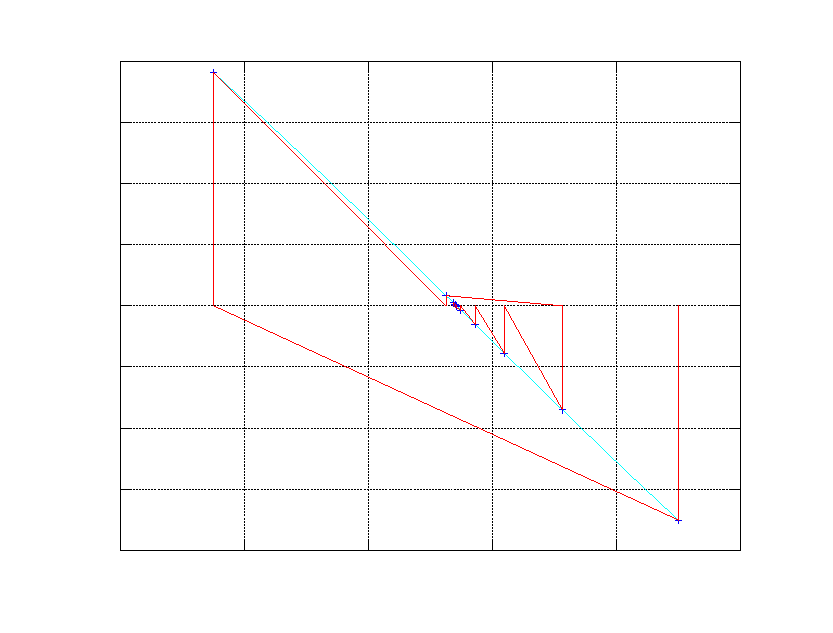
\includegraphics{RadiciEquazione/bisectionPlotOutput}}%
    \gplfronttext
  \end{picture}%
\endgroup

\end{center}

\begin{exercise}
Implementare il metodo di bisezione ed applicarlo alla funzione $\sin(x)$ 
con intervallo iniziale $[-0.1, 7]$, in modo da avere due zeri nell'
intervallo di confidenza, ed una tollerenza $tol_{X} = 10^{-14}$.
\end{exercise}
Per l'implementazione del codice vedere \nameref{sec:bisectionIterativeMethod}.
\begin{lstlisting}
octave:51> [x, i, imax, ascisse] = bisectionMethod('sin', -0.1, 7, e^-14)
x =  6.28318557739258e+00
i =  1.70000000000000e+01
imax =  2.40000000000000e+01
ascisse =
 Columns 1 through 3:
   3.45000000000000e+00   5.22500000000000e+00   6.11250000000000e+00
 Columns 4 through 6:
   6.55625000000000e+00   6.33437500000000e+00   6.22343750000000e+00
 Columns 7 through 9:
   6.27890625000000e+00   6.30664062500000e+00   6.29277343750000e+00
 Columns 10 through 12:
   6.28583984375000e+00   6.28237304687500e+00   6.28410644531250e+00
 Columns 13 through 15:
   6.28323974609375e+00   6.28280639648438e+00   6.28302307128906e+00
 Columns 16 and 17:
   6.28313140869141e+00   6.28318557739258e+00
octave:52> xsin = min(ascisse):0.01:max(ascisse)
octave:53> ysin = feval('sin', xsin)
octave:54> [prepX, prepY] = prepareForPlottingMethodSegments(ascisse, "sin", "")
octave:55> plot(xsin, ysin, "c", ascisse, feval('sin', ascisse), "b+", prepX,
prepY, "r") 
octave:56> print 'bisectionWithTwoRootsPlotOutput.tex' '-dTex' '-S800, 600'
\end{lstlisting}
Si raggiunge la tolleranza richiesta in 17 passi, sette in meno delle iterazioni massime possibili. 
Questo l'output del comando \emph{octave:56}:
\begin{center}
% GNUPLOT: LaTeX picture with Postscript
\begingroup
  \makeatletter
  \providecommand\color[2][]{%
    \GenericError{(gnuplot) \space\space\space\@spaces}{%
      Package color not loaded in conjunction with
      terminal option `colourtext'%
    }{See the gnuplot documentation for explanation.%
    }{Either use 'blacktext' in gnuplot or load the package
      color.sty in LaTeX.}%
    \renewcommand\color[2][]{}%
  }%
  \providecommand\includegraphics[2][]{%
    \GenericError{(gnuplot) \space\space\space\@spaces}{%
      Package graphicx or graphics not loaded%
    }{See the gnuplot documentation for explanation.%
    }{The gnuplot epslatex terminal needs graphicx.sty or graphics.sty.}%
    \renewcommand\includegraphics[2][]{}%
  }%
  \providecommand\rotatebox[2]{#2}%
  \@ifundefined{ifGPcolor}{%
    \newif\ifGPcolor
    \GPcolortrue
  }{}%
  \@ifundefined{ifGPblacktext}{%
    \newif\ifGPblacktext
    \GPblacktexttrue
  }{}%
  % define a \g@addto@macro without @ in the name:
  \let\gplgaddtomacro\g@addto@macro
  % define empty templates for all commands taking text:
  \gdef\gplbacktext{}%
  \gdef\gplfronttext{}%
  \makeatother
  \ifGPblacktext
    % no textcolor at all
    \def\colorrgb#1{}%
    \def\colorgray#1{}%
  \else
    % gray or color?
    \ifGPcolor
      \def\colorrgb#1{\color[rgb]{#1}}%
      \def\colorgray#1{\color[gray]{#1}}%
      \expandafter\def\csname LTw\endcsname{\color{white}}%
      \expandafter\def\csname LTb\endcsname{\color{black}}%
      \expandafter\def\csname LTa\endcsname{\color{black}}%
      \expandafter\def\csname LT0\endcsname{\color[rgb]{1,0,0}}%
      \expandafter\def\csname LT1\endcsname{\color[rgb]{0,1,0}}%
      \expandafter\def\csname LT2\endcsname{\color[rgb]{0,0,1}}%
      \expandafter\def\csname LT3\endcsname{\color[rgb]{1,0,1}}%
      \expandafter\def\csname LT4\endcsname{\color[rgb]{0,1,1}}%
      \expandafter\def\csname LT5\endcsname{\color[rgb]{1,1,0}}%
      \expandafter\def\csname LT6\endcsname{\color[rgb]{0,0,0}}%
      \expandafter\def\csname LT7\endcsname{\color[rgb]{1,0.3,0}}%
      \expandafter\def\csname LT8\endcsname{\color[rgb]{0.5,0.5,0.5}}%
    \else
      % gray
      \def\colorrgb#1{\color{black}}%
      \def\colorgray#1{\color[gray]{#1}}%
      \expandafter\def\csname LTw\endcsname{\color{white}}%
      \expandafter\def\csname LTb\endcsname{\color{black}}%
      \expandafter\def\csname LTa\endcsname{\color{black}}%
      \expandafter\def\csname LT0\endcsname{\color{black}}%
      \expandafter\def\csname LT1\endcsname{\color{black}}%
      \expandafter\def\csname LT2\endcsname{\color{black}}%
      \expandafter\def\csname LT3\endcsname{\color{black}}%
      \expandafter\def\csname LT4\endcsname{\color{black}}%
      \expandafter\def\csname LT5\endcsname{\color{black}}%
      \expandafter\def\csname LT6\endcsname{\color{black}}%
      \expandafter\def\csname LT7\endcsname{\color{black}}%
      \expandafter\def\csname LT8\endcsname{\color{black}}%
    \fi
  \fi
  \setlength{\unitlength}{0.0500bp}%
  \begin{picture}(7680.00,5760.00)%
    \gplgaddtomacro\gplbacktext{%
      \colorrgb{0.00,0.00,0.00}%
      \put(866,634){\makebox(0,0)[r]{\strut{}-1}}%
      \colorrgb{0.00,0.00,0.00}%
      \put(866,1304){\makebox(0,0)[r]{\strut{}-0.8}}%
      \colorrgb{0.00,0.00,0.00}%
      \put(866,1975){\makebox(0,0)[r]{\strut{}-0.6}}%
      \colorrgb{0.00,0.00,0.00}%
      \put(866,2645){\makebox(0,0)[r]{\strut{}-0.4}}%
      \colorrgb{0.00,0.00,0.00}%
      \put(866,3316){\makebox(0,0)[r]{\strut{}-0.2}}%
      \colorrgb{0.00,0.00,0.00}%
      \put(866,3986){\makebox(0,0)[r]{\strut{}0}}%
      \colorrgb{0.00,0.00,0.00}%
      \put(866,4657){\makebox(0,0)[r]{\strut{}0.2}}%
      \colorrgb{0.00,0.00,0.00}%
      \put(866,5327){\makebox(0,0)[r]{\strut{}0.4}}%
      \colorrgb{0.00,0.00,0.00}%
      \put(998,414){\makebox(0,0){\strut{}3}}%
      \colorrgb{0.00,0.00,0.00}%
      \put(1742,414){\makebox(0,0){\strut{}3.5}}%
      \colorrgb{0.00,0.00,0.00}%
      \put(2486,414){\makebox(0,0){\strut{}4}}%
      \colorrgb{0.00,0.00,0.00}%
      \put(3230,414){\makebox(0,0){\strut{}4.5}}%
      \colorrgb{0.00,0.00,0.00}%
      \put(3974,414){\makebox(0,0){\strut{}5}}%
      \colorrgb{0.00,0.00,0.00}%
      \put(4718,414){\makebox(0,0){\strut{}5.5}}%
      \colorrgb{0.00,0.00,0.00}%
      \put(5462,414){\makebox(0,0){\strut{}6}}%
      \colorrgb{0.00,0.00,0.00}%
      \put(6206,414){\makebox(0,0){\strut{}6.5}}%
      \colorrgb{0.00,0.00,0.00}%
      \put(6950,414){\makebox(0,0){\strut{}7}}%
    }%
    \gplgaddtomacro\gplfronttext{%
    }%
    \gplbacktext
    \put(0,0){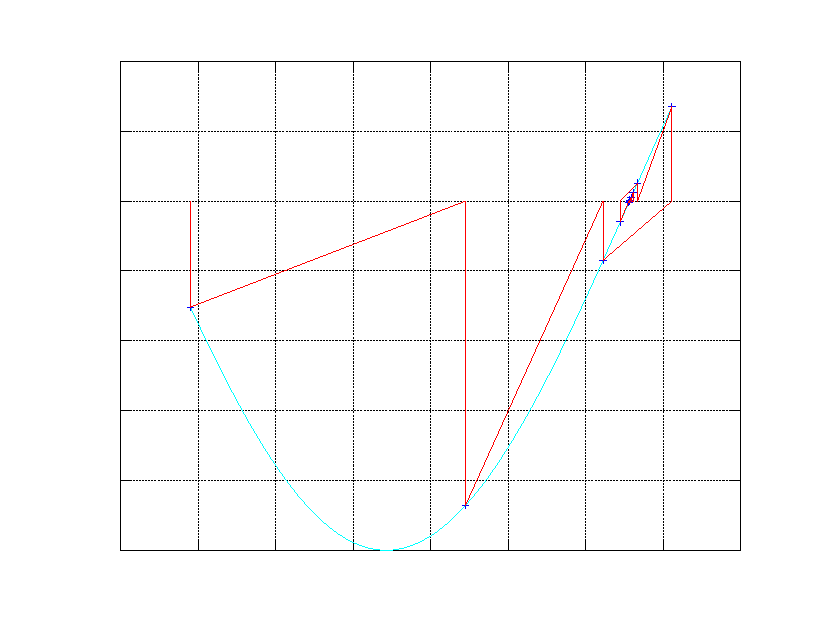
\includegraphics{RadiciEquazione/bisectionWithTwoRootsPlotOutput}}%
    \gplfronttext
  \end{picture}%
\endgroup

\end{center}

Da questo esercizio si vede che il metodo di bisezione converge comunque
ad una radice (in questa applicazione a $2\pi$), anche nel caso in cui
nell'intervallo di confidenza ci sono pi\`u zeri della funzione.





\section{Metodo di Newton}
\label{sec:metodoDiNewton}

\begin{exercise}
Implementare il metodo di newton ed applicarlo alla funzione \emph{singleZero},
con innesco iniziale $x_{0} = 7$, una tollerenza assoluta e relativa
$tol_{X} = rTol_{X} = 10^{-14}$ ed un numero massimo di iterazioni
$i_{max} = 10^{2}$.
\end{exercise}
Per l'implementazione del codice vedere \nameref{sec:newtonIterativeMethod}.
\begin{lstlisting}
octave:112> [x, i, ascisse] = newtonMethod('singleZero','singleZeroDerivative',7, 1e2, 1e-14, 1e-14, 'incrementCriterion') 
x =  3.40512483795333e+00
i =  5.00000000000000e+00
ascisse = [too long to report here]
octave:113> xSingleZero = min(ascisse)-1:0.1:max(ascisse)+1
octave:114> ySingleZero = invokeDelegate('singleZero', xSingleZero)
octave:115> [prepX, prepY] = prepareForPlottingMethodSegments(ascisse, 'invokeDelegate', 'singleZero')
octave:116> plot(xSingleZero, ySingleZero, "c", ascisse, invokeDelegate('singleZero', ascisse), "b+", prepX, prepY, "r")
octave:117> grid
octave:118> print 'newtonPlotOutput.tex' '-dTex' '-S800, 600'
\end{lstlisting}
Si raggiunge la tolleranza richiesta in 5 passi. Questo l'output del comando
\emph{octave:118}:
\begin{center}
% GNUPLOT: LaTeX picture with Postscript
\begingroup
  \makeatletter
  \providecommand\color[2][]{%
    \GenericError{(gnuplot) \space\space\space\@spaces}{%
      Package color not loaded in conjunction with
      terminal option `colourtext'%
    }{See the gnuplot documentation for explanation.%
    }{Either use 'blacktext' in gnuplot or load the package
      color.sty in LaTeX.}%
    \renewcommand\color[2][]{}%
  }%
  \providecommand\includegraphics[2][]{%
    \GenericError{(gnuplot) \space\space\space\@spaces}{%
      Package graphicx or graphics not loaded%
    }{See the gnuplot documentation for explanation.%
    }{The gnuplot epslatex terminal needs graphicx.sty or graphics.sty.}%
    \renewcommand\includegraphics[2][]{}%
  }%
  \providecommand\rotatebox[2]{#2}%
  \@ifundefined{ifGPcolor}{%
    \newif\ifGPcolor
    \GPcolortrue
  }{}%
  \@ifundefined{ifGPblacktext}{%
    \newif\ifGPblacktext
    \GPblacktexttrue
  }{}%
  % define a \g@addto@macro without @ in the name:
  \let\gplgaddtomacro\g@addto@macro
  % define empty templates for all commands taking text:
  \gdef\gplbacktext{}%
  \gdef\gplfronttext{}%
  \makeatother
  \ifGPblacktext
    % no textcolor at all
    \def\colorrgb#1{}%
    \def\colorgray#1{}%
  \else
    % gray or color?
    \ifGPcolor
      \def\colorrgb#1{\color[rgb]{#1}}%
      \def\colorgray#1{\color[gray]{#1}}%
      \expandafter\def\csname LTw\endcsname{\color{white}}%
      \expandafter\def\csname LTb\endcsname{\color{black}}%
      \expandafter\def\csname LTa\endcsname{\color{black}}%
      \expandafter\def\csname LT0\endcsname{\color[rgb]{1,0,0}}%
      \expandafter\def\csname LT1\endcsname{\color[rgb]{0,1,0}}%
      \expandafter\def\csname LT2\endcsname{\color[rgb]{0,0,1}}%
      \expandafter\def\csname LT3\endcsname{\color[rgb]{1,0,1}}%
      \expandafter\def\csname LT4\endcsname{\color[rgb]{0,1,1}}%
      \expandafter\def\csname LT5\endcsname{\color[rgb]{1,1,0}}%
      \expandafter\def\csname LT6\endcsname{\color[rgb]{0,0,0}}%
      \expandafter\def\csname LT7\endcsname{\color[rgb]{1,0.3,0}}%
      \expandafter\def\csname LT8\endcsname{\color[rgb]{0.5,0.5,0.5}}%
    \else
      % gray
      \def\colorrgb#1{\color{black}}%
      \def\colorgray#1{\color[gray]{#1}}%
      \expandafter\def\csname LTw\endcsname{\color{white}}%
      \expandafter\def\csname LTb\endcsname{\color{black}}%
      \expandafter\def\csname LTa\endcsname{\color{black}}%
      \expandafter\def\csname LT0\endcsname{\color{black}}%
      \expandafter\def\csname LT1\endcsname{\color{black}}%
      \expandafter\def\csname LT2\endcsname{\color{black}}%
      \expandafter\def\csname LT3\endcsname{\color{black}}%
      \expandafter\def\csname LT4\endcsname{\color{black}}%
      \expandafter\def\csname LT5\endcsname{\color{black}}%
      \expandafter\def\csname LT6\endcsname{\color{black}}%
      \expandafter\def\csname LT7\endcsname{\color{black}}%
      \expandafter\def\csname LT8\endcsname{\color{black}}%
    \fi
  \fi
  \setlength{\unitlength}{0.0500bp}%
  \begin{picture}(7680.00,5760.00)%
    \gplgaddtomacro\gplbacktext{%
      \colorrgb{0.00,0.00,0.00}%
      \put(866,634){\makebox(0,0)[r]{\strut{}-10}}%
      \colorrgb{0.00,0.00,0.00}%
      \put(866,1304){\makebox(0,0)[r]{\strut{}0}}%
      \colorrgb{0.00,0.00,0.00}%
      \put(866,1975){\makebox(0,0)[r]{\strut{}10}}%
      \colorrgb{0.00,0.00,0.00}%
      \put(866,2645){\makebox(0,0)[r]{\strut{}20}}%
      \colorrgb{0.00,0.00,0.00}%
      \put(866,3316){\makebox(0,0)[r]{\strut{}30}}%
      \colorrgb{0.00,0.00,0.00}%
      \put(866,3986){\makebox(0,0)[r]{\strut{}40}}%
      \colorrgb{0.00,0.00,0.00}%
      \put(866,4657){\makebox(0,0)[r]{\strut{}50}}%
      \colorrgb{0.00,0.00,0.00}%
      \put(866,5327){\makebox(0,0)[r]{\strut{}60}}%
      \colorrgb{0.00,0.00,0.00}%
      \put(998,414){\makebox(0,0){\strut{}2}}%
      \colorrgb{0.00,0.00,0.00}%
      \put(1990,414){\makebox(0,0){\strut{}3}}%
      \colorrgb{0.00,0.00,0.00}%
      \put(2982,414){\makebox(0,0){\strut{}4}}%
      \colorrgb{0.00,0.00,0.00}%
      \put(3974,414){\makebox(0,0){\strut{}5}}%
      \colorrgb{0.00,0.00,0.00}%
      \put(4966,414){\makebox(0,0){\strut{}6}}%
      \colorrgb{0.00,0.00,0.00}%
      \put(5958,414){\makebox(0,0){\strut{}7}}%
      \colorrgb{0.00,0.00,0.00}%
      \put(6950,414){\makebox(0,0){\strut{}8}}%
    }%
    \gplgaddtomacro\gplfronttext{%
    }%
    \gplbacktext
    \put(0,0){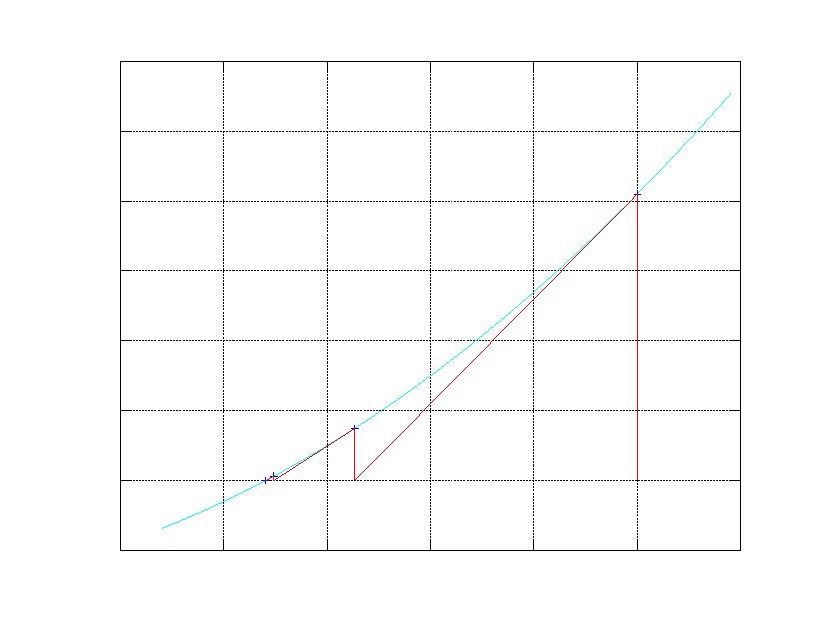
\includegraphics{RadiciEquazione/newton/newtonPlotOutput}}%
    \gplfronttext
  \end{picture}%
\endgroup

\end{center}

\begin{oss}
Per l'applicazione eseguita sopra ho utilizzato il criterio di arresto
\emph{incremento}, il metodo converge, ma posso studiare il condizionamento che
affetta ogni valutazione della precisione richiesta. Questo il codice che
dimostra questo condizionamento, comparando l'applicazione del metodo usando il
criterio di arresto per \emph{residuo}:
\begin{lstlisting}
[x, i, incAscisse, incChecked] = newtonMethod('singleZero','singleZeroDerivative', 7, 1e2, 10^(-14), 10^(-14), 'incrementCriterion');
octave:138> i
i =  5.00000000000000e+00
octave:139> errors = errorMonitor(incAscisse)
errors =
   4.12195121951219e+00   9.88875669244497e+00   8.93522817393261e+01   8.95110152113953e+03   9.18666331414061e+07   7.66765947567831e+15
octave:140> incChecked 
incChecked =
   2.73333333333333e+00   7.83682983682984e-01   7.70978577615202e-02   7.60913136916397e-04   7.41319183816813e-08   8.88178419700125e-16
octave:141> [x, i, resAscisse, resChecked] = newtonMethod('singleZero','singleZeroDerivative', 7, 1e2, 10^(-14), 10^(-14), 'residueCriterion');
octave:142> resChecked 
resChecked =
   2.73333333333333e+00   7.83682983682984e-01   7.70978577615201e-02   7.60913136916414e-04   7.41319183470686e-08   6.82317562092805e-16
octave:143> i
i =  5.00000000000000e+00
\end{lstlisting}
Si osserva che i valori utilizzati nel controllo per il raggiungimento della
precisione richiesta sono uguali tranne l'ultimo, il metodo che usa il criterio
\emph{residueCriterion} \`e pi\`u accurato, in quanto non \`e affetto dalla
cancellazione numerica (per l'ultima coppia di ascisse trovata il fattore di
amplificazione \`e $k = 7.66765947567831e+15$). 

I due metodi utilizzano comunque
lo stesso numero di passi per convergere alla soluzione.
\end{oss}

\begin{oss}
Posso effettuare una nuova comparazione: se chiedo una precisione di $tol_{X}
= 1e-16$, si osserva che il metodo non converge se si utilizza il criterio di 
arresto per \emph{incremento}, mentre converge usando il criterio per
\emph{residuo}. Questo il codice che dimostra quanto detto:
\begin{lstlisting}
octave:5> [x, i]=newtonMethod('singleZero','singleZeroDerivative', 7, 1e2, 10^(-16), 10^(-16),'incrementCriterion');
Il metodo non converge.
octave:6> [x, i]=newtonMethod('singleZero','singleZeroDerivative', 7, 1e2, 10^(-16), 10^(-16),'residueCriterion');
octave:7> i
i =  6
octave:8>
\end{lstlisting}
A parit\`a di numero massimo di passi, il secondo criterio permette al metodo di
convergere.
\end{oss}


\begin{exercise}
Implementare il metodo di newton ed applicarlo alla funzione \emph{functionWithNoRealZero},
con innesco iniziale $x_{0} = 2.5$, una tollerenza assoluta e relativa
$tol_{X} = rTol_{X} = 10^{-14}$ ed un numero massimo di iterazioni
$i_{max} = 7$.
\end{exercise}
Per l'implementazione del codice vedere \nameref{sec:newtonIterativeMethod}.
\begin{lstlisting}
octave:112> [x, i, ascisse] =
newtonMethod('functionWithNoRealZero','functionWithNoRealZeroDerivative', 2.5, 7, 1e-14, 1e-14, 'incrementCriterion') 
Il metodo non converge.
x = -3.18786023393994e+00
i =  7.00000000000000e+00
ascisse = [too long to report here]
octave:113> xNoZero = min(ascisse)-1:0.1:max(ascisse)+1
octave:114> yNoZero = invokeDelegate('functionWithNoRealZero', xNoZero)
octave:115> [prepX, prepY] = prepareForPlottingMethodSegments(ascisse, 'invokeDelegate', 'functionWithNoRealZero')
octave:116> plot(xNoZero, yNoZero, "c", ascisse,invokeDelegate('functionWithNoRealZero', ascisse), "b+", prepX, prepY, "r")
octave:117> grid
octave:118> print 'newtonNoZeroPlotOutput.tex' '-dTex' '-S800, 600'
\end{lstlisting}
Non si raggiunge la convergenza, infatti vengono fatti il massimo possibile
dei passi fissati dal parametro $i_{max}$. Questo l'output del comando \emph{octave:118}:
\begin{center}
% GNUPLOT: LaTeX picture with Postscript
\begingroup
  \makeatletter
  \providecommand\color[2][]{%
    \GenericError{(gnuplot) \space\space\space\@spaces}{%
      Package color not loaded in conjunction with
      terminal option `colourtext'%
    }{See the gnuplot documentation for explanation.%
    }{Either use 'blacktext' in gnuplot or load the package
      color.sty in LaTeX.}%
    \renewcommand\color[2][]{}%
  }%
  \providecommand\includegraphics[2][]{%
    \GenericError{(gnuplot) \space\space\space\@spaces}{%
      Package graphicx or graphics not loaded%
    }{See the gnuplot documentation for explanation.%
    }{The gnuplot epslatex terminal needs graphicx.sty or graphics.sty.}%
    \renewcommand\includegraphics[2][]{}%
  }%
  \providecommand\rotatebox[2]{#2}%
  \@ifundefined{ifGPcolor}{%
    \newif\ifGPcolor
    \GPcolortrue
  }{}%
  \@ifundefined{ifGPblacktext}{%
    \newif\ifGPblacktext
    \GPblacktexttrue
  }{}%
  % define a \g@addto@macro without @ in the name:
  \let\gplgaddtomacro\g@addto@macro
  % define empty templates for all commands taking text:
  \gdef\gplbacktext{}%
  \gdef\gplfronttext{}%
  \makeatother
  \ifGPblacktext
    % no textcolor at all
    \def\colorrgb#1{}%
    \def\colorgray#1{}%
  \else
    % gray or color?
    \ifGPcolor
      \def\colorrgb#1{\color[rgb]{#1}}%
      \def\colorgray#1{\color[gray]{#1}}%
      \expandafter\def\csname LTw\endcsname{\color{white}}%
      \expandafter\def\csname LTb\endcsname{\color{black}}%
      \expandafter\def\csname LTa\endcsname{\color{black}}%
      \expandafter\def\csname LT0\endcsname{\color[rgb]{1,0,0}}%
      \expandafter\def\csname LT1\endcsname{\color[rgb]{0,1,0}}%
      \expandafter\def\csname LT2\endcsname{\color[rgb]{0,0,1}}%
      \expandafter\def\csname LT3\endcsname{\color[rgb]{1,0,1}}%
      \expandafter\def\csname LT4\endcsname{\color[rgb]{0,1,1}}%
      \expandafter\def\csname LT5\endcsname{\color[rgb]{1,1,0}}%
      \expandafter\def\csname LT6\endcsname{\color[rgb]{0,0,0}}%
      \expandafter\def\csname LT7\endcsname{\color[rgb]{1,0.3,0}}%
      \expandafter\def\csname LT8\endcsname{\color[rgb]{0.5,0.5,0.5}}%
    \else
      % gray
      \def\colorrgb#1{\color{black}}%
      \def\colorgray#1{\color[gray]{#1}}%
      \expandafter\def\csname LTw\endcsname{\color{white}}%
      \expandafter\def\csname LTb\endcsname{\color{black}}%
      \expandafter\def\csname LTa\endcsname{\color{black}}%
      \expandafter\def\csname LT0\endcsname{\color{black}}%
      \expandafter\def\csname LT1\endcsname{\color{black}}%
      \expandafter\def\csname LT2\endcsname{\color{black}}%
      \expandafter\def\csname LT3\endcsname{\color{black}}%
      \expandafter\def\csname LT4\endcsname{\color{black}}%
      \expandafter\def\csname LT5\endcsname{\color{black}}%
      \expandafter\def\csname LT6\endcsname{\color{black}}%
      \expandafter\def\csname LT7\endcsname{\color{black}}%
      \expandafter\def\csname LT8\endcsname{\color{black}}%
    \fi
  \fi
  \setlength{\unitlength}{0.0500bp}%
  \begin{picture}(7680.00,5760.00)%
    \gplgaddtomacro\gplbacktext{%
      \colorrgb{0.00,0.00,0.00}%
      \put(866,634){\makebox(0,0)[r]{\strut{}0}}%
      \colorrgb{0.00,0.00,0.00}%
      \put(866,1807){\makebox(0,0)[r]{\strut{}5}}%
      \colorrgb{0.00,0.00,0.00}%
      \put(866,2981){\makebox(0,0)[r]{\strut{}10}}%
      \colorrgb{0.00,0.00,0.00}%
      \put(866,4154){\makebox(0,0)[r]{\strut{}15}}%
      \colorrgb{0.00,0.00,0.00}%
      \put(866,5327){\makebox(0,0)[r]{\strut{}20}}%
      \colorrgb{0.00,0.00,0.00}%
      \put(998,414){\makebox(0,0){\strut{}-6}}%
      \colorrgb{0.00,0.00,0.00}%
      \put(2188,414){\makebox(0,0){\strut{}-4}}%
      \colorrgb{0.00,0.00,0.00}%
      \put(3379,414){\makebox(0,0){\strut{}-2}}%
      \colorrgb{0.00,0.00,0.00}%
      \put(4569,414){\makebox(0,0){\strut{}0}}%
      \colorrgb{0.00,0.00,0.00}%
      \put(5760,414){\makebox(0,0){\strut{}2}}%
      \colorrgb{0.00,0.00,0.00}%
      \put(6950,414){\makebox(0,0){\strut{}4}}%
    }%
    \gplgaddtomacro\gplfronttext{%
    }%
    \gplbacktext
    \put(0,0){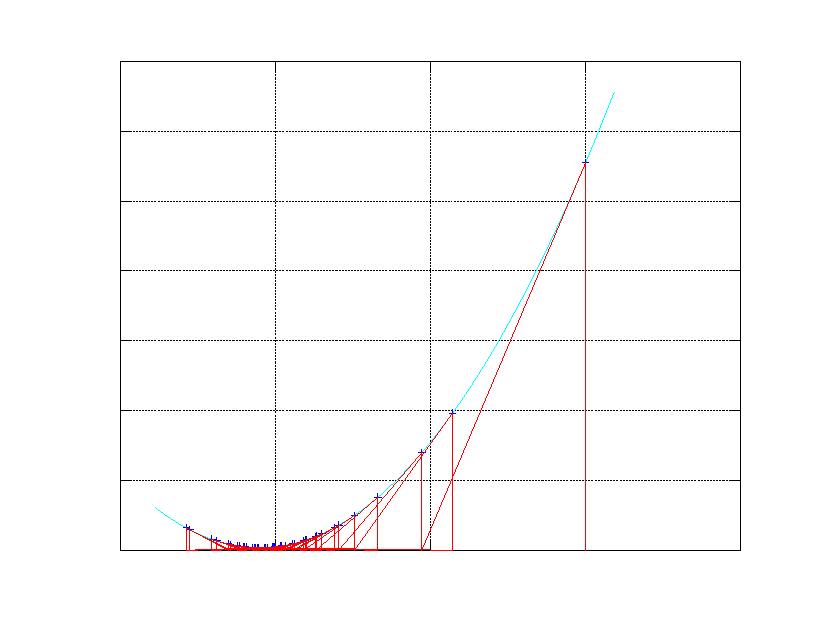
\includegraphics{RadiciEquazione/newton/newtonNoZeroPlotOutput}}%
    \gplfronttext
  \end{picture}%
\endgroup

\end{center}

\begin{exercise}[2.4]
\label{exercise:newtonLoopStartingPoint}
Per il testo dell'esercizio consultare il libro di testo.
\end{exercise}
Per l'implementazione del codice vedere \nameref{sec:newtonIterativeMethod}.

Nel primo caso studio il punto di innesco $x_{0} = 10$:
\begin{lstlisting}
octave:112> [x, i, ascisse] =
newtonMethod('functionNewtonRecursion','functionNewtonRecursionDerivative', 10, 5e1, 1e-14, 1e-14, 'incrementCriterion') 
x =  2.23606797749979e+00
i =  9.00000000000000e+00
ascisse = [too long to report here]
octave:113> xNoZero = min(ascisse)-1:0.1:max(ascisse)+1
octave:114> yNoZero = invokeDelegate('functionNewtonRecursion', xNoZero)
octave:115> [prepX, prepY] = prepareForPlottingMethodSegments(ascisse, 'invokeDelegate', 'functionNewtonRecursion')
octave:116> plot(xNoZero, yNoZero, "c", ascisse,invokeDelegate('functionNewtonRecursion', ascisse), "b+", prepX, prepY, "r")
octave:117> grid
octave:118> print 'newtonRecursivePlotOutput.tex' '-dTex' '-S800, 600'
\end{lstlisting}
Si raggiunge la convergenza con 9 passi. Questo l'output del comando
\emph{octave:118}:
\begin{center}
% GNUPLOT: LaTeX picture with Postscript
\begingroup
  \makeatletter
  \providecommand\color[2][]{%
    \GenericError{(gnuplot) \space\space\space\@spaces}{%
      Package color not loaded in conjunction with
      terminal option `colourtext'%
    }{See the gnuplot documentation for explanation.%
    }{Either use 'blacktext' in gnuplot or load the package
      color.sty in LaTeX.}%
    \renewcommand\color[2][]{}%
  }%
  \providecommand\includegraphics[2][]{%
    \GenericError{(gnuplot) \space\space\space\@spaces}{%
      Package graphicx or graphics not loaded%
    }{See the gnuplot documentation for explanation.%
    }{The gnuplot epslatex terminal needs graphicx.sty or graphics.sty.}%
    \renewcommand\includegraphics[2][]{}%
  }%
  \providecommand\rotatebox[2]{#2}%
  \@ifundefined{ifGPcolor}{%
    \newif\ifGPcolor
    \GPcolortrue
  }{}%
  \@ifundefined{ifGPblacktext}{%
    \newif\ifGPblacktext
    \GPblacktexttrue
  }{}%
  % define a \g@addto@macro without @ in the name:
  \let\gplgaddtomacro\g@addto@macro
  % define empty templates for all commands taking text:
  \gdef\gplbacktext{}%
  \gdef\gplfronttext{}%
  \makeatother
  \ifGPblacktext
    % no textcolor at all
    \def\colorrgb#1{}%
    \def\colorgray#1{}%
  \else
    % gray or color?
    \ifGPcolor
      \def\colorrgb#1{\color[rgb]{#1}}%
      \def\colorgray#1{\color[gray]{#1}}%
      \expandafter\def\csname LTw\endcsname{\color{white}}%
      \expandafter\def\csname LTb\endcsname{\color{black}}%
      \expandafter\def\csname LTa\endcsname{\color{black}}%
      \expandafter\def\csname LT0\endcsname{\color[rgb]{1,0,0}}%
      \expandafter\def\csname LT1\endcsname{\color[rgb]{0,1,0}}%
      \expandafter\def\csname LT2\endcsname{\color[rgb]{0,0,1}}%
      \expandafter\def\csname LT3\endcsname{\color[rgb]{1,0,1}}%
      \expandafter\def\csname LT4\endcsname{\color[rgb]{0,1,1}}%
      \expandafter\def\csname LT5\endcsname{\color[rgb]{1,1,0}}%
      \expandafter\def\csname LT6\endcsname{\color[rgb]{0,0,0}}%
      \expandafter\def\csname LT7\endcsname{\color[rgb]{1,0.3,0}}%
      \expandafter\def\csname LT8\endcsname{\color[rgb]{0.5,0.5,0.5}}%
    \else
      % gray
      \def\colorrgb#1{\color{black}}%
      \def\colorgray#1{\color[gray]{#1}}%
      \expandafter\def\csname LTw\endcsname{\color{white}}%
      \expandafter\def\csname LTb\endcsname{\color{black}}%
      \expandafter\def\csname LTa\endcsname{\color{black}}%
      \expandafter\def\csname LT0\endcsname{\color{black}}%
      \expandafter\def\csname LT1\endcsname{\color{black}}%
      \expandafter\def\csname LT2\endcsname{\color{black}}%
      \expandafter\def\csname LT3\endcsname{\color{black}}%
      \expandafter\def\csname LT4\endcsname{\color{black}}%
      \expandafter\def\csname LT5\endcsname{\color{black}}%
      \expandafter\def\csname LT6\endcsname{\color{black}}%
      \expandafter\def\csname LT7\endcsname{\color{black}}%
      \expandafter\def\csname LT8\endcsname{\color{black}}%
    \fi
  \fi
  \setlength{\unitlength}{0.0500bp}%
  \begin{picture}(7680.00,5760.00)%
    \gplgaddtomacro\gplbacktext{%
      \colorrgb{0.00,0.00,0.00}%
      \put(866,634){\makebox(0,0)[r]{\strut{}-500}}%
      \colorrgb{0.00,0.00,0.00}%
      \put(866,1807){\makebox(0,0)[r]{\strut{}0}}%
      \colorrgb{0.00,0.00,0.00}%
      \put(866,2981){\makebox(0,0)[r]{\strut{}500}}%
      \colorrgb{0.00,0.00,0.00}%
      \put(866,4154){\makebox(0,0)[r]{\strut{}1000}}%
      \colorrgb{0.00,0.00,0.00}%
      \put(866,5327){\makebox(0,0)[r]{\strut{}1500}}%
      \colorrgb{0.00,0.00,0.00}%
      \put(998,414){\makebox(0,0){\strut{}0}}%
      \colorrgb{0.00,0.00,0.00}%
      \put(1990,414){\makebox(0,0){\strut{}2}}%
      \colorrgb{0.00,0.00,0.00}%
      \put(2982,414){\makebox(0,0){\strut{}4}}%
      \colorrgb{0.00,0.00,0.00}%
      \put(3974,414){\makebox(0,0){\strut{}6}}%
      \colorrgb{0.00,0.00,0.00}%
      \put(4966,414){\makebox(0,0){\strut{}8}}%
      \colorrgb{0.00,0.00,0.00}%
      \put(5958,414){\makebox(0,0){\strut{}10}}%
      \colorrgb{0.00,0.00,0.00}%
      \put(6950,414){\makebox(0,0){\strut{}12}}%
    }%
    \gplgaddtomacro\gplfronttext{%
    }%
    \gplbacktext
    \put(0,0){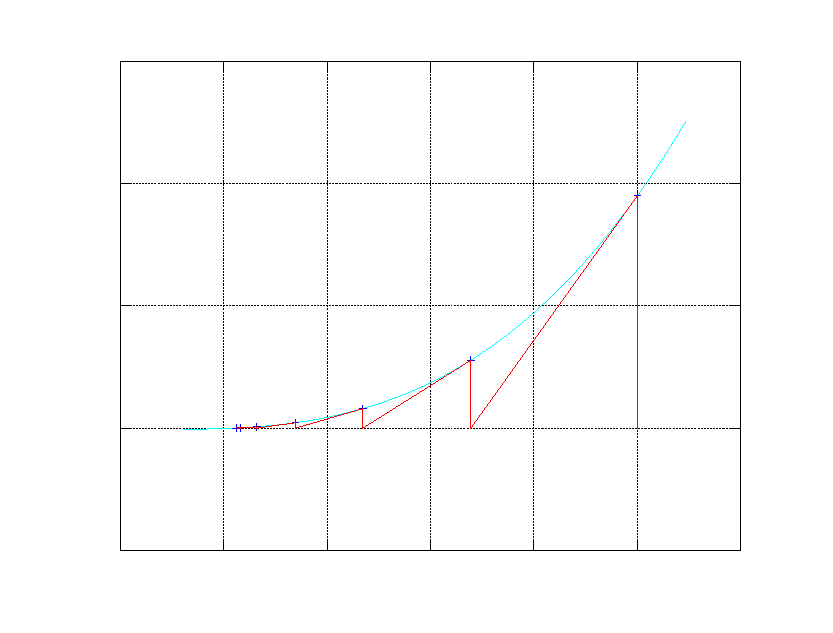
\includegraphics{RadiciEquazione/newton/newtonRecursivePlotOutput}}%
    \gplfronttext
  \end{picture}%
\endgroup

\end{center}

Nel secondo caso studio il punto di innesco $x_{0} = 1$:
\begin{lstlisting}
octave:112> [x, i, ascisse] =
newtonMethod('functionNewtonRecursion','functionNewtonRecursionDerivative', 1, 5e1, 1e-14, 1e-14, 'incrementCriterion') 
Il metodo non converge.
x = -1.00000000000000e+00
i =  5.00000000000000e+01
ascisse = [too long to report here]
octave:113> xNoZero = min(ascisse)-1:0.1:max(ascisse)+1
octave:114> yNoZero = invokeDelegate('functionNewtonRecursion', xNoZero)
octave:115> [prepX, prepY] = prepareForPlottingMethodSegments(ascisse, 'invokeDelegate', 'functionNewtonRecursion')
octave:116> plot(xNoZero, yNoZero, "c", ascisse,invokeDelegate('functionNewtonRecursion', ascisse), "b+", prepX, prepY, "r")
octave:117> grid
octave:118> print 'newtonRecursiveNotConvergencePlotOutput.tex' '-dTex' '-S800,600'
\end{lstlisting}
Il metodo non converge creando una finestra come si vede nel grafico. Questo
l'output del comando \emph{octave:118}:
\begin{center}
% GNUPLOT: LaTeX picture with Postscript
\begingroup
  \makeatletter
  \providecommand\color[2][]{%
    \GenericError{(gnuplot) \space\space\space\@spaces}{%
      Package color not loaded in conjunction with
      terminal option `colourtext'%
    }{See the gnuplot documentation for explanation.%
    }{Either use 'blacktext' in gnuplot or load the package
      color.sty in LaTeX.}%
    \renewcommand\color[2][]{}%
  }%
  \providecommand\includegraphics[2][]{%
    \GenericError{(gnuplot) \space\space\space\@spaces}{%
      Package graphicx or graphics not loaded%
    }{See the gnuplot documentation for explanation.%
    }{The gnuplot epslatex terminal needs graphicx.sty or graphics.sty.}%
    \renewcommand\includegraphics[2][]{}%
  }%
  \providecommand\rotatebox[2]{#2}%
  \@ifundefined{ifGPcolor}{%
    \newif\ifGPcolor
    \GPcolortrue
  }{}%
  \@ifundefined{ifGPblacktext}{%
    \newif\ifGPblacktext
    \GPblacktexttrue
  }{}%
  % define a \g@addto@macro without @ in the name:
  \let\gplgaddtomacro\g@addto@macro
  % define empty templates for all commands taking text:
  \gdef\gplbacktext{}%
  \gdef\gplfronttext{}%
  \makeatother
  \ifGPblacktext
    % no textcolor at all
    \def\colorrgb#1{}%
    \def\colorgray#1{}%
  \else
    % gray or color?
    \ifGPcolor
      \def\colorrgb#1{\color[rgb]{#1}}%
      \def\colorgray#1{\color[gray]{#1}}%
      \expandafter\def\csname LTw\endcsname{\color{white}}%
      \expandafter\def\csname LTb\endcsname{\color{black}}%
      \expandafter\def\csname LTa\endcsname{\color{black}}%
      \expandafter\def\csname LT0\endcsname{\color[rgb]{1,0,0}}%
      \expandafter\def\csname LT1\endcsname{\color[rgb]{0,1,0}}%
      \expandafter\def\csname LT2\endcsname{\color[rgb]{0,0,1}}%
      \expandafter\def\csname LT3\endcsname{\color[rgb]{1,0,1}}%
      \expandafter\def\csname LT4\endcsname{\color[rgb]{0,1,1}}%
      \expandafter\def\csname LT5\endcsname{\color[rgb]{1,1,0}}%
      \expandafter\def\csname LT6\endcsname{\color[rgb]{0,0,0}}%
      \expandafter\def\csname LT7\endcsname{\color[rgb]{1,0.3,0}}%
      \expandafter\def\csname LT8\endcsname{\color[rgb]{0.5,0.5,0.5}}%
    \else
      % gray
      \def\colorrgb#1{\color{black}}%
      \def\colorgray#1{\color[gray]{#1}}%
      \expandafter\def\csname LTw\endcsname{\color{white}}%
      \expandafter\def\csname LTb\endcsname{\color{black}}%
      \expandafter\def\csname LTa\endcsname{\color{black}}%
      \expandafter\def\csname LT0\endcsname{\color{black}}%
      \expandafter\def\csname LT1\endcsname{\color{black}}%
      \expandafter\def\csname LT2\endcsname{\color{black}}%
      \expandafter\def\csname LT3\endcsname{\color{black}}%
      \expandafter\def\csname LT4\endcsname{\color{black}}%
      \expandafter\def\csname LT5\endcsname{\color{black}}%
      \expandafter\def\csname LT6\endcsname{\color{black}}%
      \expandafter\def\csname LT7\endcsname{\color{black}}%
      \expandafter\def\csname LT8\endcsname{\color{black}}%
    \fi
  \fi
  \setlength{\unitlength}{0.0500bp}%
  \begin{picture}(7680.00,5760.00)%
    \gplgaddtomacro\gplbacktext{%
      \colorrgb{0.00,0.00,0.00}%
      \put(866,634){\makebox(0,0)[r]{\strut{}-6}}%
      \colorrgb{0.00,0.00,0.00}%
      \put(866,1416){\makebox(0,0)[r]{\strut{}-4}}%
      \colorrgb{0.00,0.00,0.00}%
      \put(866,2198){\makebox(0,0)[r]{\strut{}-2}}%
      \colorrgb{0.00,0.00,0.00}%
      \put(866,2981){\makebox(0,0)[r]{\strut{}0}}%
      \colorrgb{0.00,0.00,0.00}%
      \put(866,3763){\makebox(0,0)[r]{\strut{}2}}%
      \colorrgb{0.00,0.00,0.00}%
      \put(866,4545){\makebox(0,0)[r]{\strut{}4}}%
      \colorrgb{0.00,0.00,0.00}%
      \put(866,5327){\makebox(0,0)[r]{\strut{}6}}%
      \colorrgb{0.00,0.00,0.00}%
      \put(998,414){\makebox(0,0){\strut{}-2}}%
      \colorrgb{0.00,0.00,0.00}%
      \put(1742,414){\makebox(0,0){\strut{}-1.5}}%
      \colorrgb{0.00,0.00,0.00}%
      \put(2486,414){\makebox(0,0){\strut{}-1}}%
      \colorrgb{0.00,0.00,0.00}%
      \put(3230,414){\makebox(0,0){\strut{}-0.5}}%
      \colorrgb{0.00,0.00,0.00}%
      \put(3974,414){\makebox(0,0){\strut{}0}}%
      \colorrgb{0.00,0.00,0.00}%
      \put(4718,414){\makebox(0,0){\strut{}0.5}}%
      \colorrgb{0.00,0.00,0.00}%
      \put(5462,414){\makebox(0,0){\strut{}1}}%
      \colorrgb{0.00,0.00,0.00}%
      \put(6206,414){\makebox(0,0){\strut{}1.5}}%
      \colorrgb{0.00,0.00,0.00}%
      \put(6950,414){\makebox(0,0){\strut{}2}}%
    }%
    \gplgaddtomacro\gplfronttext{%
    }%
    \gplbacktext
    \put(0,0){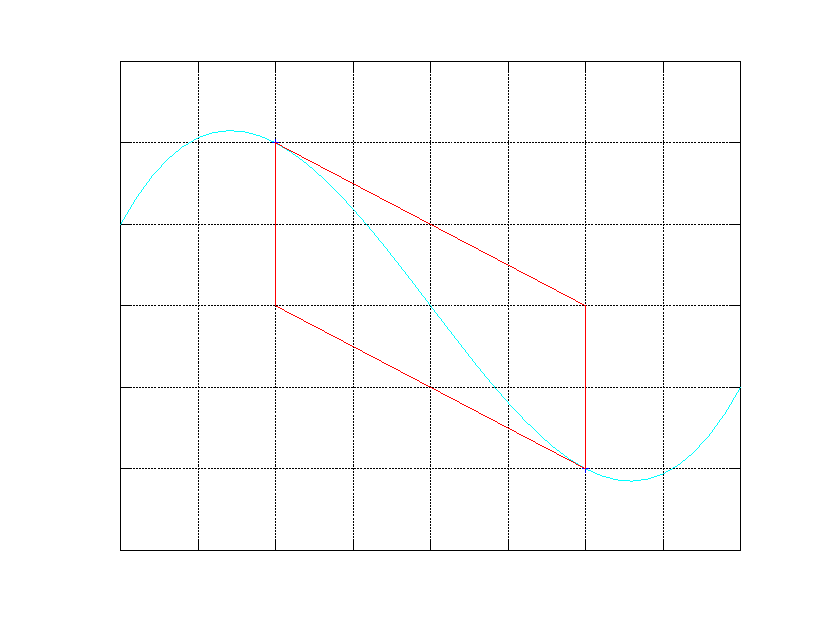
\includegraphics{RadiciEquazione/newton/newtonRecursiveNotConvergencePlotOutput}}%
    \gplfronttext
  \end{picture}%
\endgroup

\end{center}

\chapter{Sorgenti Octave}

\section{Metodo iterativo}
\label{sec:iterativeMethodToSQRT2}
\lstinputlisting{listings/chapterOne/iterative.m}

\section{Utility functions}
\subsection{invokeDelegate}
\lstinputlisting{listings/chapterTwo/invokeDelegate.m}

\subsection{prepareForPlottingMethodSegments}
\lstinputlisting{listings/chapterTwo/prepareForPlottingMethodSegments.m}

\section{Metodo di bisezione}
\label{sec:bisectionIterativeMethod}
\lstinputlisting{listings/chapterTwo/bisectionMethod.m}

\section{Metodo di Newton}
\label{sec:newtonIterativeMethod}
Questa implementazione utilizza il criterio di arresto esposto nell'
\emph{Osservazione 2.3} nel caso di radici semplici.

Una osservazione sul numero di passi effettuati: per la mia implementazione
vale $i = length(ascisse) + 2$ in quanto nel ciclo \emph{while} colleziono
$length(ascisse)$ valori, pi\`u uno per il valore di innesco iniziale, pi\`u uno
per l'ultimo valore appena usciti dal ciclo \emph{while}.
\lstinputlisting{listings/chapterTwo/newtonMethod.m}

\section{Varianti del metodo di Newton}

\subsection{Molteplicit\`a dello zero nota}
\label{subsec:newtonMethodMultKnown}
Questa implementazione utilizza il criterio di arresto esposto nell'
\emph{Osservazione 2.3} nel caso di radici semplici.
\lstinputlisting{listings/chapterTwo/newtonMethodMoltKnown.m}

\subsection{Molteplicit\`a dello zero nota con criterio di arresto lineare}
\label{subsec:newtonMethodMultKnownLinearStopCriteria}
Questa implementazione utilizza il criterio di arresto esposto nell'
\emph{Osservazione 2.3} nel caso di radici multiple, ovvero il criterio di
arresto sar\`a dato da:
\begin{displaymath}
	|x_{i+1} - x_{i}| \leq \frac{1-c}{c}tol_{X}
\end{displaymath}
Ricavo in modo dinamico la costante $c$, usando le tre iterate pi\`u recenti:
\begin{displaymath}
	c \approx \frac{|x_{i} - x_{i-1}|}{|x_{i-1} - x_{i-2}|}
\end{displaymath}
Posso usare questa approssimazione in quanto $m > 1$ per ipotesi del problema,
quindi per il \emph{Teorema 2.2}, il metodo di Newton converge linearmente verso zeri
multipli, 
condizione necessaria per applicare questo criterio di arresto.
\lstinputlisting{listings/chapterTwo/newtonMethodMoltKnownLinearCriteria.m}


\chapter*{Help di Octave}

\section{Helps for \nameref{sec:metodoDiBisezione} section}

Riporto qui alcune righe di help per le funzioni che verranno utilizzate 
pi\`u spesso in questo capitolo:

\begin{lstlisting}
octave:1> help poly
`poly' is a function from the file /usr/share/octave/3.2.3/m/polynomial/poly.m

 -- Function File:  poly (A)
     If A is a square N-by-N matrix, `poly (A)' is the row vector of
     the coefficients of `det (z * eye (N) - a)', the characteristic
     polynomial of A.  As an example we can use this to find the
     eigenvalues of A as the roots of `poly (A)'.
          roots(poly(eye(3)))
          => 1.00000 - 0.00000i
          => 1.00000 + 0.00000i
     In real-life examples you should, however, use the `eig' function
     for computing eigenvalues.

     If X is a vector, `poly (X)' is a vector of coefficients of the
     polynomial whose roots are the elements of X.  That is, of C is a
     polynomial, then the elements of `D = roots (poly (C))' are
     contained in C.  The vectors C and D are, however, not equal due
     to sorting and numerical errors.

     See also: eig, roots
\end{lstlisting}

\begin{lstlisting}
octave:1> help ones
`ones' is a built-in function

 -- Built-in Function:  ones (X)
 -- Built-in Function:  ones (N, M)
 -- Built-in Function:  ones (N, M, K, ...)
 -- Built-in Function:  ones (..., CLASS)
     Return a matrix or N-dimensional array whose elements are all 1.
     The arguments are handled the same as the arguments for `eye'.

     If you need to create a matrix whose values are all the same, you
     should use an expression like

          val_matrix = val * ones (n, m)
\end{lstlisting}

\begin{lstlisting}
octave:1> help polyval
`polyval' is a function from the file /usr/share/octave/3.2.3/m/polynomial/polyval.m

 -- Function File: Y = polyval (P, X)
 -- Function File: Y = polyval (P, X, [], MU)
     Evaluate the polynomial at of the specified values for X.  When MU
     is present evaluate the polynomial for (X-MU(1))/MU(2).  If X is a
     vector or matrix, the polynomial is evaluated for each of the
     elements of X.

 -- Function File: [Y, DY] = polyval (P, X, S)
 -- Function File: [Y, DY] = polyval (P, X, S, MU)
     In addition to evaluating the polynomial, the second output
     represents the prediction interval, Y +/- DY, which contains at
     least 50% of the future predictions.  To calculate the prediction
     interval, the structured variable S, originating form `polyfit',
     must be present.

     See also: polyfit, polyvalm, poly, roots, conv, deconv, residue,
     filter, polyderiv, polyinteg
\end{lstlisting}

\begin{lstlisting}
octave:14> help ceil
`ceil' is a built-in function

 -- Mapping Function:  ceil (X)
     Return the smallest integer not less than X.  This is equivalent to
     rounding towards positive infinity.  If X is complex, return `ceil
     (real (X)) + ceil (imag (X)) * I'.
          ceil ([-2.7, 2.7])
            =>  -2   3

     See also: floor, round, fix
\end{lstlisting}


\end{document} 
